% Provenance (never printed): cycle 3 / 6e "La planete Terre" (water in the
% ground, groundwater, springs and wells; resource); see
% sources/book1/PROVENANCE.md. Book 1, grade 6, chapter 5.
% Vocabulary guard: "sediment" not before g7.4; the water cycle is recalled
% from the physics book (prose only).
\chapter{L'eau souterraine}\label{ch:g6:water-underground}

Par une chaude journée d'été, les champs sont secs et les ruisseaux sont
bas. Pourtant, au pied d'une \omterm{def:g1:landscapes-around-us:landform}{colline}, l'eau continue de sortir du sol,
froide et claire, comme tout l'hiver, et remplit un bassin. Il n'a pas plu
depuis des semaines. D'où vient cette eau, et comment sort-elle de la
\omterm{def:g3:stones-pebbles-sand:rock}{roche}~?

\begin{omfigure}
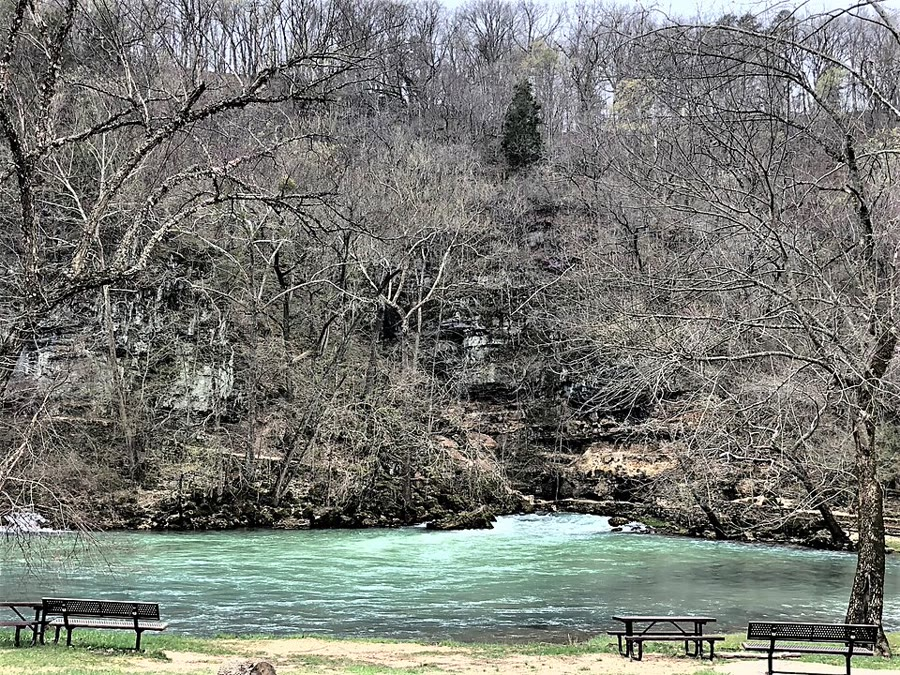
\includegraphics[width=0.72\linewidth]{images/book1/g6-big-spring.jpg}

{\small Une \omterm{def:g6:water-underground:spring}{source} jaillit au pied d'un escarpement rocheux et remplit un
bassin~: Big Spring, dans le Missouri (États-Unis). (Photo~: Johnston9494,
CC BY-SA 4.0, via Wikimedia Commons.)}
% ledger: commons:big-spring
\end{omfigure}

\begin{recall}
Presque toute l'eau de la Terre est de l'\omterm{def:g2:water-on-earth:salt-fresh}{eau salée}~; l'\omterm{def:g2:water-on-earth:salt-fresh}{eau douce} n'en est
qu'une petite partie, stockée surtout sous forme de glace et sous le sol
(\cref{ch:g2:water-on-earth}). Des \omterm{def:g3:stones-pebbles-sand:rock}{roches} comme le grès et le calcaire sont
faites de grains ou de coquilles collés entre eux, tandis que l'argile et
l'argilite sont faites de particules très fines
(\cref{ch:g6:rocks-and-minerals}). Dans le livre de physique, tu as suivi
l'eau tout au long du cycle de l'eau~: elle s'évapore des \omterm{def:g2:water-on-earth:ocean}{mers}, se
condense en \omterm{def:g4:clouds-rain-snow:cloud}{nuages} et retombe sous forme de \omterm{def:g4:clouds-rain-snow:precipitation}{pluie} ou de \omterm{def:g4:clouds-rain-snow:precipitation}{neige}.
\end{recall}

\section{La pluie s'infiltre}

Quand la \omterm{def:g4:clouds-rain-snow:precipitation}{pluie} tombe sur les terres, l'eau peut prendre trois chemins. Une
partie s'évapore et retourne dans l'air. Une partie s'écoule à la surface,
le long des pentes, jusque dans les ruisseaux et les \omterm{def:g1:landscapes-around-us:water}{rivières}~: c'est le
\emph{ruissellement}. Le reste s'infiltre dans le sol.

\begin{definition}[Infiltration]\label{def:g6:water-underground:infiltration}
L'\emph{infiltration}\index{infiltration} est la pénétration de l'eau de
\omterm{def:g4:clouds-rain-snow:precipitation}{pluie}, ou de la \omterm{def:g4:clouds-rain-snow:precipitation}{neige} fondue, dans le sol, à travers la terre et jusque
dans les \omterm{def:g3:stones-pebbles-sand:rock}{roches}.
\end{definition}

La quantité d'eau qui s'infiltre dépend du terrain. Sur une pente raide,
sur un sol nu ou dur, sur une route ou un parking, ou quand le sol est déjà
gorgé d'eau, la plus grande partie de l'eau ruisselle. Sur une pente douce,
sous l'herbe et les arbres, sur un sol sableux, une plus grande partie a le
temps de s'infiltrer.

\begin{omfigure}
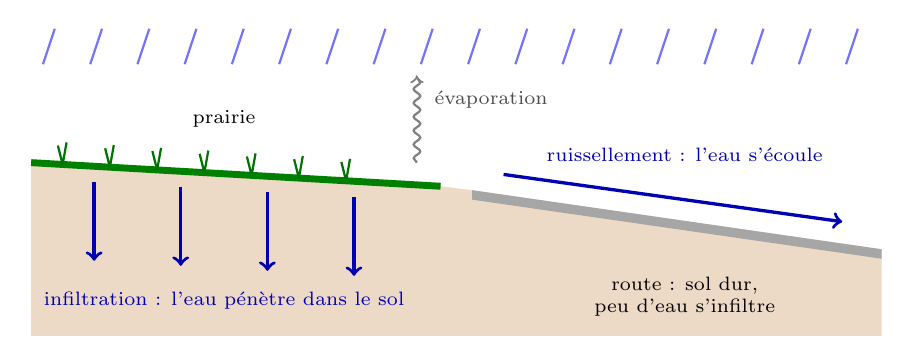
\begin{tikzpicture}[x=1cm, y=1cm]
  % rain
  \foreach \x in {0.3,0.9,...,10.5} \draw[blue!55, thick] (\x,3.9) -- (\x-0.15,3.45);
  % ground: field on the left (gentle), road and town on the right
  \fill[brown!30] (0,0) -- (0,2.2) -- (5.2,1.9) -- (5.6,1.85) -- (10.8,1.1) -- (10.8,0) -- cycle;
  \draw[green!50!black, line width=2.5pt] (0,2.2) -- (5.2,1.9);
  \fill[gray!70] (5.6,1.85) -- (10.8,1.1) -- (10.8,0.98) -- (5.6,1.73) -- cycle;
  \foreach \x in {0.4,1.0,...,4.6} \draw[green!45!black, thick] (\x,{2.2-0.058*\x}) -- ++(0.05,0.28) (\x,{2.2-0.058*\x}) -- ++(-0.06,0.24);
  % infiltration arrows in the field
  \foreach \x in {0.8,1.9,3.0,4.1} \draw[->, blue!70!black, very thick] (\x,{2.0-0.058*\x}) -- ++(0,-1.0);
  \node[font=\scriptsize, blue!70!black, align=center, fill=brown!30] at (2.45,0.45) {infiltration~: l'eau pénètre dans le sol};
  % run-off on the road
  \draw[->, blue!70!black, very thick] (6.0,2.05) -- (10.3,1.45);
  \node[font=\scriptsize, blue!70!black, align=center] at (8.3,2.3) {ruissellement~: l'eau s'écoule};
  \node[font=\scriptsize, align=center] at (8.3,0.5) {route~: sol dur,\\ peu d'eau s'infiltre};
  \node[font=\scriptsize] at (2.45,2.75) {prairie};
  % evaporation
  \draw[->, gray, thick, decorate, decoration={snake, amplitude=1.2pt, segment length=5pt}] (4.9,2.2) -- (4.9,3.3);
  \node[font=\scriptsize, gray!60!black, anchor=west] at (5.0,3.0) {évaporation};
\end{tikzpicture}

{\small Les trois chemins de l'eau de \omterm{def:g4:clouds-rain-snow:precipitation}{pluie}. Dans la prairie, une grande
partie s'infiltre~; sur la route, la plus grande partie ruisselle.}
\end{omfigure}

\section{Roches poreuses et roches perméables}

Regarde à la loupe une poignée de \omterm{def:g3:stones-pebbles-sand:sand}{sable} sec~: entre les grains, il y a de
minuscules espaces vides. Verse de l'eau dessus, et l'eau remplit ces
espaces. Beaucoup de \omterm{def:g3:stones-pebbles-sand:rock}{roches} sont ainsi~: elles sont pleines de petits trous
entre leurs grains, ou de fines fissures.

\begin{definition}[Porosité]\label{def:g6:water-underground:porosity}
Les \emph{pores}\index{pore} d'une \omterm{def:g3:stones-pebbles-sand:rock}{roche} sont les espaces vides entre ses
grains et dans ses fissures. Une \omterm{def:g3:stones-pebbles-sand:rock}{roche} qui a des pores est
\emph{poreuse}\index{poreux}. Sa \emph{porosité}\index{porosite@porosité}
est la part de son volume occupée par les pores, exprimée en pourcentage.
\end{definition}

\begin{definition}[Perméabilité]\label{def:g6:water-underground:permeability}
Une \omterm{def:g3:stones-pebbles-sand:rock}{roche} est \emph{perméable}\index{permeable@perméable} quand l'eau peut
la traverser, parce que ses \omterm{def:g6:water-underground:porosity}{pores} sont assez grands et reliés les uns aux
autres. Elle est \emph{imperméable}\index{impermeable@imperméable} quand
l'eau ne peut pas la traverser. La
\emph{perméabilité}\index{permeabilite@perméabilité} indique avec quelle
facilité l'eau traverse une \omterm{def:g3:stones-pebbles-sand:rock}{roche}.
\end{definition}

Ces deux idées ne sont pas les mêmes. L'argile est très \omterm{def:g6:water-underground:porosity}{poreuse}~: la
moitié de son volume est faite de \omterm{def:g6:water-underground:porosity}{pores}. Mais ses \omterm{def:g6:water-underground:porosity}{pores} sont si minuscules
que l'eau y reste collée~: l'argile est \emph{\omterm{def:g6:water-underground:permeability}{imperméable}}. Le \omterm{def:g3:stones-pebbles-sand:sand}{sable} a
moins de \omterm{def:g6:water-underground:porosity}{pores} que l'argile, mais ils sont larges et reliés entre eux~: le
\omterm{def:g3:stones-pebbles-sand:sand}{sable} est \emph{\omterm{def:g6:water-underground:permeability}{perméable}}. Un granite sans fissures n'a presque aucun
\omterm{def:g6:water-underground:porosity}{pore}.
% ledger: heath:porosity

\begin{omfigure}
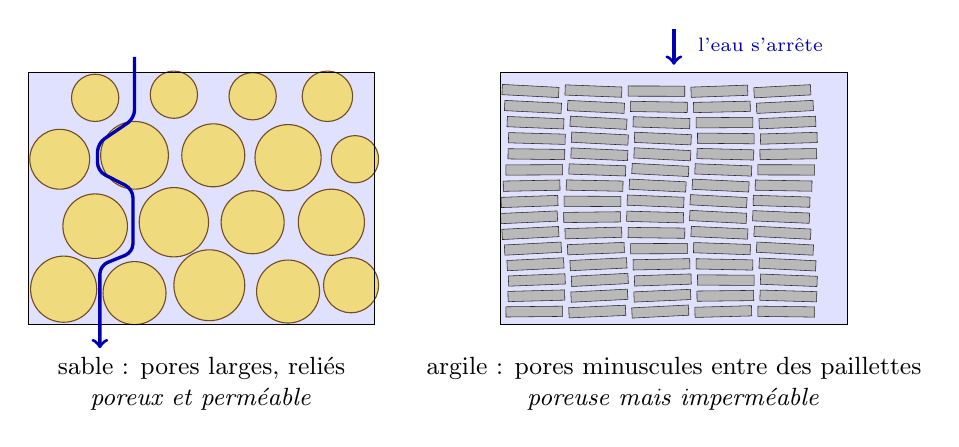
\begin{tikzpicture}
  % sand
  \begin{scope}
    \fill[blue!12] (0,0) rectangle (4.4,3.2);
    \foreach \x/\y/\r in {0.45/0.45/0.42, 1.35/0.4/0.4, 2.3/0.5/0.45, 3.3/0.42/0.4, 4.1/0.5/0.35,
                         0.85/1.25/0.41, 1.85/1.3/0.44, 2.85/1.3/0.4, 3.85/1.3/0.42,
                         0.4/2.1/0.38, 1.35/2.15/0.43, 2.35/2.15/0.4, 3.3/2.12/0.42, 4.15/2.1/0.3,
                         0.85/2.88/0.3, 1.85/2.92/0.3, 2.85/2.9/0.3, 3.8/2.9/0.32}
      \fill[yellow!55!brown!60, draw=brown!60!black] (\x,\y) circle (\r);
    \draw (0,0) rectangle (4.4,3.2);
    \draw[->, blue!70!black, very thick, rounded corners=3pt] (1.35,3.4) -- (1.35,2.62) -- (0.88,2.3) -- (0.88,1.95) -- (1.33,1.72) -- (1.33,0.92) -- (0.91,0.75) -- (0.91,-0.3);
    \node[font=\small, align=center] at (2.2,-0.75) {sable~: pores larges, reliés\\ \emph{poreux et perméable}};
  \end{scope}
  % clay
  \begin{scope}[xshift=6.0cm]
    \fill[blue!12] (0,0) rectangle (4.4,3.2);
    \foreach \y in {0.1,0.3,...,3.0}
      \foreach \x in {0.05,0.85,...,3.7}
        \fill[gray!55, draw=gray!30!black, line width=0.2pt, rotate around={{3*sin(57*\x+91*\y)}:(\x+0.36,\y+0.06)}]
          ({\x+0.05*sin(200*\y)},\y) rectangle ++(0.72,0.13);
    \draw (0,0) rectangle (4.4,3.2);
    \draw[->, blue!70!black, very thick] (2.2,3.75) -- (2.2,3.3);
    \node[font=\scriptsize, blue!70!black] at (3.3,3.55) {l'eau s'arrête};
    \node[font=\small, align=center] at (2.2,-0.75) {argile~: pores minuscules entre des paillettes\\ \emph{poreuse mais imperméable}};
  \end{scope}
\end{tikzpicture}

{\small Les \omterm{def:g6:water-underground:porosity}{pores} (en bleu) entre les grains d'un \omterm{def:g3:stones-pebbles-sand:sand}{sable} et entre les
paillettes d'une argile, très agrandis. L'eau trouve un chemin à travers le
\omterm{def:g3:stones-pebbles-sand:sand}{sable}~; dans l'argile, elle reste collée.}
\end{omfigure}

Le tableau donne la \omterm{def:g6:water-underground:porosity}{porosité} de quelques matériaux, et la part de l'eau qui
s'en écoule d'elle-même quand ils sont pleins d'eau. Le reste reste collé
aux grains.

\begin{center}\small
\begin{tabular}{|l|c|c|}
\hline
\textbf{matériau} & \textbf{\omterm{def:g6:water-underground:porosity}{porosité} (\%)} & \textbf{eau qui s'écoule (\%)} \\
\hline
sol & 55 & 40 \\
argile & 50 & 2 \\
\omterm{def:g3:stones-pebbles-sand:sand}{sable} & 25 & 22 \\
\omterm{def:g3:stones-pebbles-sand:pebble}{graviers} & 20 & 19 \\
calcaire & 20 & 18 \\
grès & 11 & 6 \\
granite & 0.1 & 0.09 \\
\hline
\end{tabular}
\end{center}
% ledger: heath:porosity

\begin{method}[Quelle quantité d'eau une roche contient-elle~?]\label{met:g6:water-underground:volume}
\begin{enumerate}
  \item Trouve le volume de la \omterm{def:g3:stones-pebbles-sand:rock}{roche} (pour un bloc~: longueur $\times$
        largeur $\times$ hauteur).
  \item Multiplie par la \omterm{def:g6:water-underground:porosity}{porosité} et divise par 100~: tu obtiens le volume
        des \omterm{def:g6:water-underground:porosity}{pores}, donc l'eau que contient la \omterm{def:g3:stones-pebbles-sand:rock}{roche} quand elle est pleine.
  \item Pour l'eau qui s'écoule, utilise le second pourcentage de la même
        façon. (1~mètre cube, c'est 1000~litres.)
\end{enumerate}
\end{method}

\begin{example}[Un mètre cube de sable]\label{ex:g6:water-underground:sand}
Un mètre cube de \omterm{def:g3:stones-pebbles-sand:sand}{sable}, plein d'eau, contient $1000 \times 25 \div 100 =
250$~litres d'eau dans ses \omterm{def:g6:water-underground:porosity}{pores}. Parmi eux, $1000 \times 22 \div 100 = 220$
litres s'écoulent d'eux-mêmes~; 30~litres restent collés aux grains. Un
mètre cube d'argile contient deux fois plus d'eau, 500~litres, mais
seulement 20~litres s'en écoulent.
% ledger: heath:porosity
\end{example}

\begin{inthelab}[Sable ou argile~? (en classe, avec l'enseignant)]
Deux pots de fleurs percés d'un trou au fond sont posés au-dessus de deux
verres. L'un est rempli de \omterm{def:g3:stones-pebbles-sand:sand}{sable} sec, l'autre de terre argileuse sèche,
tassée. L'enseignant verse le même verre d'eau dans chacun, au même
moment. À travers le \omterm{def:g3:stones-pebbles-sand:sand}{sable}, l'eau goutte bientôt dans le verre du dessous.
Sur l'argile, l'eau reste en surface comme une flaque, et seules quelques
gouttes passent, lentement~: le \omterm{def:g3:stones-pebbles-sand:sand}{sable} est \omterm{def:g6:water-underground:permeability}{perméable}, l'argile ne l'est
pas.
\end{inthelab}

\section{L'eau souterraine et le niveau de la nappe}

Creuse un trou dans le \omterm{def:g3:stones-pebbles-sand:sand}{sable} d'une plage, à quelques pas de la \omterm{def:g2:water-on-earth:ocean}{mer}~: au
bout d'un moment, de l'eau apparaît au fond du trou. Tu as atteint
l'endroit où tous les \omterm{def:g6:water-underground:porosity}{pores} du \omterm{def:g3:stones-pebbles-sand:sand}{sable} sont pleins d'eau.
% ledger: wss:aquifer

\begin{definition}[Eau souterraine]\label{def:g6:water-underground:groundwater}
L'\emph{eau souterraine}\index{eau souterraine} est l'eau du sous-sol qui
remplit les \omterm{def:g6:water-underground:porosity}{pores} et les fissures du sol et des \omterm{def:g3:stones-pebbles-sand:rock}{roches}.
\end{definition}

\begin{definition}[Niveau de la nappe]\label{def:g6:water-underground:water-table}
Au-dessous d'une certaine profondeur, tous les \omterm{def:g6:water-underground:porosity}{pores} de la \omterm{def:g3:stones-pebbles-sand:rock}{roche} sont
pleins d'eau~: c'est la nappe d'\omterm{def:g6:water-underground:groundwater}{eau souterraine}. Le
\emph{niveau de la nappe}\index{niveau de la nappe} est le haut de cette
zone remplie d'eau. Au-dessus, les \omterm{def:g6:water-underground:porosity}{pores} contiennent de l'air et un peu
d'eau~; au-dessous, ils sont pleins d'eau.
% ledger: wss:aquifer
\end{definition}

Le \omterm{def:g6:water-underground:water-table}{niveau de la nappe} n'est pas plat. Il suit la forme du terrain, mais en
plus doux~: plus haut sous les \omterm{def:g1:landscapes-around-us:landform}{collines}, plus bas sous les \omterm{def:g1:landscapes-around-us:landform}{vallées}. Il monte
et descend aussi avec les saisons. Après une saison des \omterm{def:g4:clouds-rain-snow:precipitation}{pluies}, la \omterm{def:g4:clouds-rain-snow:precipitation}{pluie}
qui s'est infiltrée le fait monter~; après une longue saison sèche, l'eau
s'écoule lentement vers les \omterm{def:g6:water-underground:spring}{sources} et les \omterm{def:g1:landscapes-around-us:water}{rivières}, et le \omterm{def:g6:water-underground:water-table}{niveau de la
nappe} descend.

L'\omterm{def:g6:water-underground:groundwater}{eau souterraine} est un grand stock d'\omterm{def:g2:water-on-earth:salt-fresh}{eau douce}. De toute l'\omterm{def:g2:water-on-earth:salt-fresh}{eau douce}
de la Terre, environ 69~\% est de la glace et de la \omterm{def:g4:clouds-rain-snow:precipitation}{neige} permanente, et
environ 30~\% est de l'\omterm{def:g6:water-underground:groundwater}{eau souterraine}~; l'\omterm{def:g2:water-on-earth:salt-fresh}{eau douce} de tous les \omterm{def:g1:landscapes-around-us:water}{lacs} n'en
représente qu'environ un quart de pour cent. L'\omterm{def:g6:water-underground:groundwater}{eau souterraine} est plus de
cent fois plus abondante que l'\omterm{def:g2:water-on-earth:salt-fresh}{eau douce} des \omterm{def:g1:landscapes-around-us:water}{lacs}.
% ledger: wss:fresh-shares

\begin{omfigure}
\begin{tikzpicture}
  \begin{axis}[xbar, width=0.8\linewidth, height=3.9cm, bar width=8pt,
      xmin=0, xmax=85, ymin=-0.6, ymax=4.6, y dir=reverse,
      ytick={0,...,4}, yticklabels={glace et neige permanentes, eau souterraine, glace du sol et pergélisol, lacs, tout le reste},
      xlabel={pourcentage de toute l'eau douce de la Terre},
      axis x line=bottom, axis y line=left, axis line style={-},
      tick label style={font=\scriptsize}, label style={font=\small},
      nodes near coords, nodes near coords style={font=\scriptsize, anchor=west},
      point meta=explicit symbolic, enlarge y limits=false, clip=false]
    \addplot[fill=blue!35, draw=blue!60!black] table[x=pct, y=idx, meta=pct] {figdata/out/grade-6-water_table-fresh.dat};
  \end{axis}
\end{tikzpicture}

{\small Où se trouve l'\omterm{def:g2:water-on-earth:salt-fresh}{eau douce} de la Terre. Les bâtons des \omterm{def:g1:landscapes-around-us:water}{lacs} et de
tout le reste (\omterm{def:g1:landscapes-around-us:water}{rivières}, air, sol, marais, êtres vivants) sont trop courts
pour être vus.}
% ledger: wss:fresh-shares (figdata/grade-6/water_table.py, part fresh)
\end{omfigure}

\section{Sources et puits}

\begin{definition}[Source et puits]\label{def:g6:water-underground:spring}
Une \emph{source}\index{source (d'eau souterraine)} est un endroit où l'\omterm{def:g6:water-underground:groundwater}{eau
souterraine} sort d'elle-même du sol, là où le \omterm{def:g6:water-underground:water-table}{niveau de la nappe} rencontre
la surface. Un \emph{puits}\index{puits} est un trou creusé ou foré
jusqu'au-dessous du \omterm{def:g6:water-underground:water-table}{niveau de la nappe}, pour que l'\omterm{def:g6:water-underground:groundwater}{eau souterraine} en
remplisse le fond et puisse être remontée.
\end{definition}

La coupe ci-dessous traverse une \omterm{def:g1:landscapes-around-us:landform}{vallée} des collines de Varden, la région
de nos exercices. Les \omterm{def:g1:landscapes-around-us:landform}{collines} sont faites de craie, un calcaire blanc,
tendre, \omterm{def:g6:water-underground:porosity}{poreux} et \omterm{def:g6:water-underground:permeability}{perméable}. Sous la craie se trouve une couche
d'argilite, qui est \omterm{def:g6:water-underground:permeability}{imperméable}. La \omterm{def:g4:clouds-rain-snow:precipitation}{pluie} s'infiltre dans la craie, remplit
ses \omterm{def:g6:water-underground:porosity}{pores} et s'arrête sur l'argilite.

\begin{omfigure}
\begin{tikzpicture}
\begin{axis}[omsection, width=0.95\linewidth, height=7.2cm,
    xmin=0, xmax=2.8, ymin=0, ymax=560,
    xlabel={distance depuis l'extrémité sud de la coupe (km)},
    ylabel={altitude (m)},
    tick label style={font=\scriptsize}, label style={font=\small},
    clip mode=individual]
  \addplot[om lith={icsJurassic!40}{om limestone}, draw=black, line width=0.3pt, even odd rule] table {figdata/out/grade-6-water_table-unit-limestone.dat};
  \addplot[om lith={icsJurassic!15}{om shale}, draw=black, line width=0.3pt, even odd rule] table {figdata/out/grade-6-water_table-unit-shale.dat};
  \addplot[om lith={icsCretaceous!35}{om limestone}, draw=black, line width=0.3pt, even odd rule] table {figdata/out/grade-6-water_table-unit-chalk.dat};
  \addplot[lith alluvium, draw=black, line width=0.3pt, even odd rule] table {figdata/out/grade-6-water_table-unit-alluvium.dat};
  \addplot[black, thick] table {figdata/out/grade-6-water_table-ground.dat};
  \addplot[blue!75!black, very thick] table {figdata/out/grade-6-water_table-wet.dat};
  \addplot[blue!75!black, very thick, dashed] table {figdata/out/grade-6-water_table-dry.dat};
  % wells
  \addplot[fill=white, draw=black, line width=0.4pt] table {figdata/out/grade-6-water_table-well-rects.dat};
  \node[font=\scriptsize\bfseries, anchor=south east, fill=white, fill opacity=0.8, text opacity=1, inner sep=1pt] at (axis cs:1.45,401.3) {puits~A};
  \node[font=\scriptsize\bfseries, anchor=south east, fill=white, fill opacity=0.8, text opacity=1, inner sep=1pt] at (axis cs:1.7,470.3) {puits~B};
  % river and spring
  \addplot[only marks, mark=*, mark size=2.2pt, blue!75!black] table[x=s_km, y=z_m] {figdata/out/grade-6-water_table-points.dat};
  \node[font=\scriptsize, blue!70!black, anchor=south east] at (axis cs:0.215,140) {rivière};
  \node[font=\scriptsize, blue!70!black, anchor=east] at (axis cs:0.83,218) {source};
  \node[font=\scriptsize] at (axis cs:2.2,470) {craie (perméable)};
  \node[font=\scriptsize, fill=white, fill opacity=0.8, text opacity=1] at (axis cs:2.2,95) {argilite (imperméable)};
  \node[font=\scriptsize, fill=white, fill opacity=0.8, text opacity=1] at (axis cs:0.95,25) {calcaire};
  \node[font=\scriptsize, blue!70!black, fill=white, fill opacity=0.8, text opacity=1, align=center] at (axis cs:2.15,250) {niveau de la nappe~:\\ après la saison des pluies (trait plein)\\ après la saison sèche (tirets)};
\end{axis}
\end{tikzpicture}

{\small Une coupe nord--sud à travers les collines de Varden, de la \omterm{def:g1:landscapes-around-us:water}{rivière}
jusqu'en haut du versant nord (hauteurs exagérées environ 2~fois). L'eau
contenue dans la craie s'arrête sur l'argilite et sort en une \omterm{def:g6:water-underground:spring}{source} là où
la base de la craie rencontre la pente. Le \omterm{def:g6:water-underground:spring}{puits}~A atteint toujours l'eau~;
le \omterm{def:g6:water-underground:spring}{puits}~B ne l'atteint qu'après la saison des \omterm{def:g4:clouds-rain-snow:precipitation}{pluies}.}
% (figdata/grade-6/water_table.py; region model figdata/shared/region.py)
\end{omfigure}

La \omterm{def:g6:water-underground:spring}{source} coule là où la base de la craie rencontre le versant~: l'eau ne
peut pas descendre à travers l'argilite, elle s'écoule donc sur le dessus
de l'argilite et sort sur la pente. Tant qu'il y a de l'eau dans la craie
au-dessus de l'argilite, la \omterm{def:g6:water-underground:spring}{source} continue de couler, même pendant un été
sec~: voilà la réponse à la question posée au début du chapitre.

Regarde les deux \omterm{def:g6:water-underground:spring}{puits}. Le \omterm{def:g6:water-underground:spring}{puits}~A est profond de 100~m~; son fond est sous
le \omterm{def:g6:water-underground:water-table}{niveau de la nappe} en toute saison, il donne donc toujours de l'eau. Le
\omterm{def:g6:water-underground:spring}{puits}~B est encore plus profond, 105~m, mais il a été creusé plus haut sur
la \omterm{def:g1:landscapes-around-us:landform}{colline}~: son fond est sous le \omterm{def:g6:water-underground:water-table}{niveau de la nappe} après la saison des
\omterm{def:g4:clouds-rain-snow:precipitation}{pluies} et au-dessus après la saison sèche. En été, le \omterm{def:g6:water-underground:spring}{puits}~B est à sec.
Ce qui compte, ce n'est pas la profondeur d'un \omterm{def:g6:water-underground:spring}{puits}, mais de combien son
fond descend sous le niveau le plus bas de la nappe.
% (figdata/grade-6/water_table.py, part wells)

\begin{omfigure}
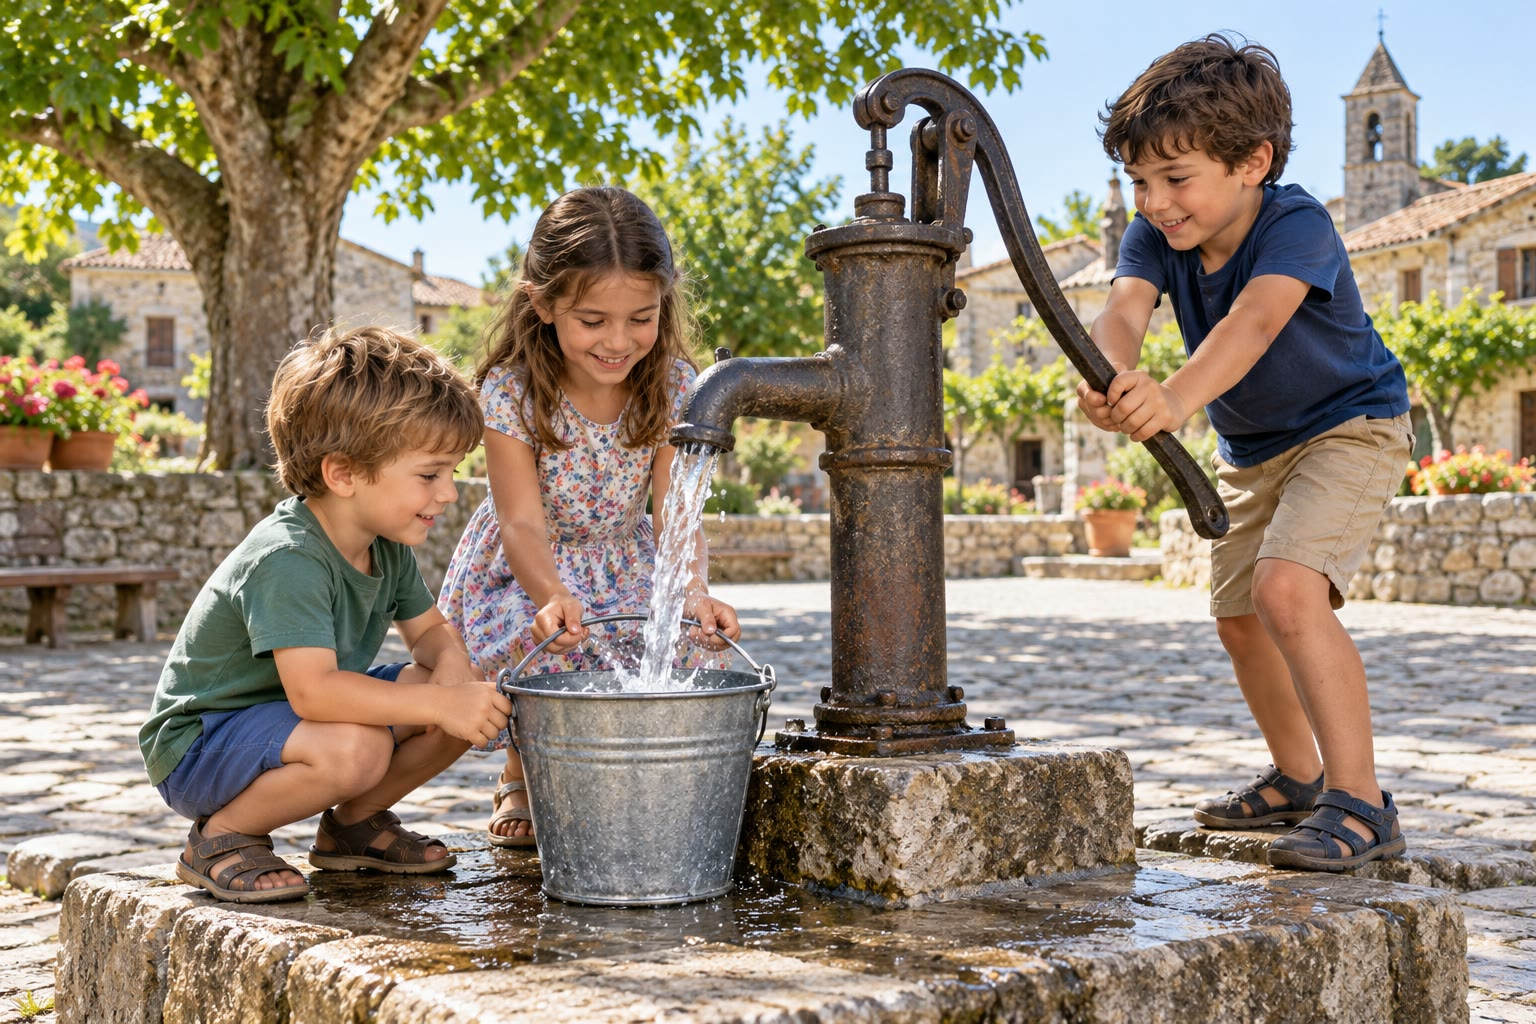
\includegraphics[width=0.6\linewidth]{images/book1/ai/g6-hand-pump.jpg}

{\small Des enfants remplissent un seau à la pompe à main d'un \omterm{def:g6:water-underground:spring}{puits} de
village. (Illustration générée par IA.)}
\end{omfigure}

\begin{remark}[Un puits peut se tarir]\label{rem:g6:water-underground:pumping}
Pomper l'eau d'un \omterm{def:g6:water-underground:spring}{puits} fait baisser le \omterm{def:g6:water-underground:water-table}{niveau de la nappe} autour de lui.
Si l'on pompe l'eau plus vite que la \omterm{def:g4:clouds-rain-snow:precipitation}{pluie} ne recharge la \omterm{def:g3:stones-pebbles-sand:rock}{roche}, le \omterm{def:g6:water-underground:water-table}{niveau
de la nappe} descend sans cesse~: le \omterm{def:g6:water-underground:spring}{puits} donne de moins en moins d'eau et
peut se tarir. Deux voisins qui pompent dans la même \omterm{def:g3:stones-pebbles-sand:rock}{roche} partagent la
même eau~: une pompe peut assécher le \omterm{def:g6:water-underground:spring}{puits} de l'autre.
% ledger: wss:aquifer
\end{remark}

\section{Les aquifères}

\begin{definition}[Aquifère]\label{def:g6:water-underground:aquifer}
Un \emph{aquifère}\index{aquifere@aquifère} est une couche de \omterm{def:g3:stones-pebbles-sand:rock}{roche}
\omterm{def:g6:water-underground:porosity}{poreuse} et \omterm{def:g6:water-underground:permeability}{perméable}, pleine d'\omterm{def:g6:water-underground:groundwater}{eau souterraine}, qui laisse cette eau
s'écouler vers les \omterm{def:g6:water-underground:spring}{sources} et les \omterm{def:g6:water-underground:spring}{puits}. La \omterm{def:g4:clouds-rain-snow:precipitation}{pluie} qui s'infiltre le
recharge.
% ledger: wss:aquifer
\end{definition}

La craie des collines de Varden est un \omterm{def:g6:water-underground:aquifer}{aquifère}~: elle est \omterm{def:g6:water-underground:porosity}{poreuse}, elle
est \omterm{def:g6:water-underground:permeability}{perméable}, et les fermes des \omterm{def:g1:landscapes-around-us:landform}{collines} y puisent leur eau. L'argilite
qui se trouve dessous n'est pas un \omterm{def:g6:water-underground:aquifer}{aquifère}~: l'eau ne peut pas la
traverser. Plus profond encore, sous l'argilite, se trouvent un calcaire et
un grès, qui peuvent eux aussi contenir de l'eau~; pour l'atteindre, il
faut forer un \omterm{def:g6:water-underground:spring}{puits} à travers toute l'argilite.

L'\omterm{def:g6:water-underground:groundwater}{eau souterraine} fait partie du cycle de l'eau. La \omterm{def:g4:clouds-rain-snow:precipitation}{pluie} s'infiltre dans
un \omterm{def:g6:water-underground:aquifer}{aquifère}~; l'\omterm{def:g6:water-underground:groundwater}{eau souterraine} circule lentement à travers les \omterm{def:g6:water-underground:porosity}{pores}~;
elle ressort aux \omterm{def:g6:water-underground:spring}{sources} et dans les \omterm{def:g1:landscapes-around-us:water}{rivières}, qui l'emportent jusqu'à la
\omterm{def:g2:water-on-earth:ocean}{mer}~; là, elle s'évapore, et retombe sous forme de \omterm{def:g4:clouds-rain-snow:precipitation}{pluie}. Prendre de l'eau
dans un \omterm{def:g6:water-underground:aquifer}{aquifère}, c'est comme prendre de l'eau dans une citerne que la
\omterm{def:g4:clouds-rain-snow:precipitation}{pluie} remplit lentement~: cela ne dure que si nous ne prenons pas plus que
ce que la \omterm{def:g4:clouds-rain-snow:precipitation}{pluie} rapporte.

\section{Garder l'eau souterraine propre}

L'eau qui s'infiltre dans le sol est filtrée en chemin~: les feuilles, les
particules de terre et les petites bêtes sont retenues par le sol et par la
\omterm{def:g3:stones-pebbles-sand:rock}{roche}. C'est pourquoi l'eau d'une \omterm{def:g6:water-underground:spring}{source} ou d'un \omterm{def:g6:water-underground:spring}{puits} paraît en général
d'une clarté de cristal. Mais les substances \emph{dissoutes} dans l'eau ne
sont pas retenues~: elles descendent avec elle jusqu'à la nappe.
% ledger: wss:gw-quality

L'\omterm{def:g6:water-underground:groundwater}{eau souterraine} peut être abîmée par ce que les gens déposent sur le
sol~: les engrais et les pesticides répandus sur les champs et les jardins,
le sel répandu sur les routes verglacées, le carburant qui fuit d'une
cuve, les déchets jetés en plein air, le débordement de fosses septiques
mal entretenues. Une fois dissoutes dans un \omterm{def:g6:water-underground:aquifer}{aquifère}, ces substances sont
difficiles à éliminer, et l'eau peut ne plus être potable sans traitement.
L'eau d'un \omterm{def:g6:water-underground:spring}{puits} doit donc être analysée avant d'être bue, et il vaut mieux
garder les engrais, le carburant et les déchets loin des \omterm{def:g6:water-underground:spring}{puits} et des
\omterm{def:g6:water-underground:spring}{sources}.
% ledger: wss:gw-quality

Les substances dissoutes voyagent avec l'\omterm{def:g6:water-underground:groundwater}{eau souterraine}. Sous le \omterm{def:g6:water-underground:water-table}{niveau
de la nappe}, l'eau descend lentement la pente~: depuis l'endroit où la
nappe est haute, sous les \omterm{def:g1:landscapes-around-us:landform}{collines}, jusqu'à l'endroit où elle est basse,
aux \omterm{def:g6:water-underground:spring}{sources} et aux \omterm{def:g1:landscapes-around-us:water}{rivières}. Une fuite qui s'infiltre ne reste donc pas là
où elle est tombée. Elle descend jusqu'à la nappe, puis dérive vers l'aval
avec l'\omterm{def:g6:water-underground:groundwater}{eau souterraine}, vers tout ce qui se trouve plus bas sur la pente.
% ledger: wss:gw-quality, wss:aquifer

\begin{omfigure}
\begin{tikzpicture}[x=1cm, y=1.15cm, font=\scriptsize]
  % ground (the chalk) and the water-filled zone under the water table
  \fill[black!6] (0,0) -- (0,4.090) -- plot[smooth] coordinates {(0.00,4.090) (1.00,4.013) (2.00,3.887) (3.00,3.692) (4.00,3.407) (5.00,3.033) (6.00,2.600) (7.00,2.167) (8.00,1.793) (9.00,1.508) (10.00,1.313) (11.00,1.187) (12.00,1.110)} -- (12,0) -- cycle;
  \fill[blue!14] (0,0) -- (0,3.190) -- plot[smooth] coordinates {(0.00,3.190) (1.00,3.185) (2.00,3.131) (3.00,3.008) (4.00,2.795) (5.00,2.493) (6.00,2.132) (7.00,1.771) (8.00,1.469) (9.00,1.256) (10.00,1.133) (11.00,1.079) (12.00,1.074)} -- (12,0) -- cycle;
  \draw[black!70, line width=0.7pt] plot[smooth] coordinates {(0.00,4.090) (1.00,4.013) (2.00,3.887) (3.00,3.692) (4.00,3.407) (5.00,3.033) (6.00,2.600) (7.00,2.167) (8.00,1.793) (9.00,1.508) (10.00,1.313) (11.00,1.187) (12.00,1.110)};
  \draw[blue!70!black, dashed, line width=0.7pt] plot[smooth] coordinates {(0.00,3.190) (1.00,3.185) (2.00,3.131) (3.00,3.008) (4.00,2.795) (5.00,2.493) (6.00,2.132) (7.00,1.771) (8.00,1.469) (9.00,1.256) (10.00,1.133) (11.00,1.079) (12.00,1.074)};
  % the spill: down to the water table, then downhill with the groundwater
  \fill[brown!70!black, opacity=0.55] (4.85,3.094) -- (5.15,2.971) -- (5.15,2.442) -- (4.85,2.544) -- cycle;
  \fill[brown!70!black, opacity=0.55] (4.85,2.514) -- (5.10,2.429) -- (5.35,2.341) -- (5.60,2.250) -- (5.85,2.158) -- (6.10,2.065) -- (6.35,1.972) -- (6.60,1.881) -- (6.85,1.792) -- (7.10,1.707) -- (7.35,1.626) -- (7.60,1.549) -- (7.85,1.478) -- (8.10,1.413) -- (8.35,1.354) -- (8.60,1.300) -- (8.85,1.252) -- (9.10,1.210) -- (9.30,1.181) -- (9.10,1.182) -- (8.85,1.190) -- (8.60,1.203) -- (8.35,1.221) -- (8.10,1.246) -- (7.85,1.277) -- (7.60,1.313) -- (7.35,1.355) -- (7.10,1.401) -- (6.85,1.486) -- (6.60,1.598) -- (6.35,1.713) -- (6.10,1.828) -- (5.85,1.945) -- (5.60,2.060) -- (5.35,2.174) -- (5.10,2.286) -- (4.85,2.394) -- cycle;
  % the leaking tank
  \draw[fill=black!35] (4.7,3.10) rectangle (5.3,3.42);
  \node[anchor=south, align=center] at (5.0,3.45) {cuve de carburant\\qui fuit};
  % groundwater flow
  \begin{scope}[blue!60!black, -{Stealth[length=2mm]}, line width=0.8pt]
    \draw (0.80,2.589) -- (2.40,2.491);
    \draw (3.40,2.334) -- (5.00,1.893);
    \draw (5.90,1.569) -- (7.50,1.009);
    \draw (8.80,0.691) -- (10.60,0.494);
  \end{scope}
  \node[blue!60!black, anchor=north] at (6.7,1.0) {l'eau souterraine descend la pente};
  % the two wells
  \draw[line width=1.6pt, black!75] (2.0,3.887) -- (2.0,2.70);
  \draw[line width=1.6pt, black!75] (8.5,1.639) -- (8.5,0.95);
  \node[anchor=south, align=center] at (2.0,3.95) {puits A\\(en amont)~: propre};
  \draw[black!50] (8.5,1.66) -- (8.5,2.30);
  \node[anchor=south, align=center] at (8.5,2.30) {puits B\\(en aval)~: pollué};
  % the stream
  \fill[blue!60] (11.55,1.13) -- (11.95,1.11) -- (11.75,1.02) -- cycle;
  \node[anchor=south] at (11.6,1.20) {ruisseau};
  \node[blue!70!black, anchor=south west] at (0.1,3.21) {niveau de la nappe};
  \node[anchor=west, black!70] at (0.15,0.25) {craie};
\end{tikzpicture}

{\small Une fuite sur un versant (croquis). Le carburant dissous descend
jusqu'au \omterm{def:g6:water-underground:water-table}{niveau de la nappe}, puis dérive vers l'aval avec l'\omterm{def:g6:water-underground:groundwater}{eau
souterraine} (flèches bleues)~: il atteint le \omterm{def:g6:water-underground:spring}{puits} B, situé plus bas sur la
pente, et finalement le ruisseau. Le \omterm{def:g6:water-underground:spring}{puits} A, en amont de la cuve, reste
propre.}
\end{omfigure}

\begin{method}[Un puits est-il menacé~?]\label{met:g6:water-underground:risk}
\begin{enumerate}
  \item Repère où le \omterm{def:g6:water-underground:water-table}{niveau de la nappe} est haut et où il est bas~: il est
        haut sous les \omterm{def:g1:landscapes-around-us:landform}{collines} et bas près des \omterm{def:g6:water-underground:spring}{sources} et des \omterm{def:g1:landscapes-around-us:water}{rivières}.
  \item L'\omterm{def:g6:water-underground:groundwater}{eau souterraine} s'écoule du haut vers le bas~: dessine son sens
        avec une flèche.
  \item Un \omterm{def:g6:water-underground:spring}{puits} ou une \omterm{def:g6:water-underground:spring}{source} situé en aval d'une \omterm{def:g6:water-underground:spring}{source} de pollution,
        sur le chemin de cette flèche, est menacé~; un \omterm{def:g6:water-underground:spring}{puits} situé en amont
        ne l'est pas.
\end{enumerate}
\end{method}

\begin{example}[Une nouvelle cuve de carburant pour la ferme]\label{ex:g6:water-underground:tank}
Une agricultrice, sur un versant de craie, boit l'eau de son propre \omterm{def:g6:water-underground:spring}{puits},
à mi-pente, et veut installer une nouvelle cuve de carburant dans l'un de
deux champs~: l'un en amont du \omterm{def:g6:water-underground:spring}{puits}, l'autre en aval, près du ruisseau.
L'\omterm{def:g6:water-underground:groundwater}{eau souterraine} s'écoule vers le bas de la pente. Une fuite dans le champ
d'amont dériverait vers le \omterm{def:g6:water-underground:spring}{puits}~; une fuite dans le champ d'aval s'en
éloignerait, vers le ruisseau. Le champ situé en aval du \omterm{def:g6:water-underground:spring}{puits} est le
meilleur choix pour le \omterm{def:g6:water-underground:spring}{puits} --- et une cuve posée sur un bac qui retient
toute fuite est encore mieux, puisque le ruisseau compte aussi.
\end{example}

\begin{inthefield}[Repérer les sources]
Pendant une promenade avec un adulte, regarde le long du pied d'une pente.
Une \omterm{def:g6:water-underground:spring}{source} se signale souvent par une tache de terre humide, une ligne
d'herbe plus verte ou de roseaux dans un champ sec, un petit ruisseau qui
part de nulle part, ou un bassin de pierre ou un abreuvoir construit pour
recueillir l'eau. Sur une \omterm{def:g2:drawing-to-map:map}{carte} de randonnée détaillée, les \omterm{def:g6:water-underground:spring}{sources} sont
marquées par un petit symbole. Observe depuis le chemin~: ne bois jamais
l'eau d'une \omterm{def:g6:water-underground:spring}{source} qui n'a pas été analysée.
\end{inthefield}

\section{Exercices}

\begin{exercise}[$\star$]\label{exo:g6:water-underground:1}
Classe ces matériaux en «~\omterm{def:g6:water-underground:permeability}{perméables}~» et «~\omterm{def:g6:water-underground:permeability}{imperméables}~»~: \omterm{def:g3:stones-pebbles-sand:sand}{sable},
argile, \omterm{def:g3:stones-pebbles-sand:pebble}{graviers}, granite sans fissures, argilite, craie.
\end{exercise}

\begin{exercise}[$\star$]\label{exo:g6:water-underground:2}
Associe chaque mot à sa définition~: \omterm{def:g6:water-underground:spring}{source}~; \omterm{def:g6:water-underground:spring}{puits}~; \omterm{def:g6:water-underground:water-table}{niveau de la
nappe}~; \omterm{def:g6:water-underground:aquifer}{aquifère}. (a) Le haut de la zone où tous les \omterm{def:g6:water-underground:porosity}{pores} sont pleins
d'eau. (b) Une couche \omterm{def:g6:water-underground:porosity}{poreuse} et \omterm{def:g6:water-underground:permeability}{perméable} qui contient de l'\omterm{def:g6:water-underground:groundwater}{eau
souterraine}. (c) Un endroit où l'\omterm{def:g6:water-underground:groundwater}{eau souterraine} sort d'elle-même. (d) Un
trou qui descend sous le \omterm{def:g6:water-underground:water-table}{niveau de la nappe}.
\end{exercise}

\begin{exercise}[$\star$]\label{exo:g6:water-underground:3}
(a) Nomme les trois chemins que peut prendre l'eau de \omterm{def:g4:clouds-rain-snow:precipitation}{pluie} quand elle
tombe sur les terres. (b) Après un orage, où l'eau ruisselle-t-elle le
plus~: sur un parking ou sur une prairie~? Pourquoi~?
\end{exercise}

\begin{exercise}[$\star$]\label{exo:g6:water-underground:4}
Vrai ou faux~? Corrige les phrases fausses. (a) Une \omterm{def:g3:stones-pebbles-sand:rock}{roche} \omterm{def:g6:water-underground:porosity}{poreuse} est
toujours \omterm{def:g6:water-underground:permeability}{perméable}. (b) Sous le \omterm{def:g6:water-underground:water-table}{niveau de la nappe}, les \omterm{def:g6:water-underground:porosity}{pores} sont pleins
d'eau. (c) Le \omterm{def:g6:water-underground:water-table}{niveau de la nappe} est plat, comme la surface d'un \omterm{def:g1:landscapes-around-us:water}{lac}.
(d) Il y a plus d'\omterm{def:g2:water-on-earth:salt-fresh}{eau douce} sous le sol que dans tous les \omterm{def:g1:landscapes-around-us:water}{lacs}.
\end{exercise}

\begin{exercise}[$\star\star$]\label{exo:g6:water-underground:5}
Un seau contient 10~litres de \omterm{def:g3:stones-pebbles-sand:sand}{sable} sec. La \omterm{def:g6:water-underground:porosity}{porosité} du \omterm{def:g3:stones-pebbles-sand:sand}{sable} est de
25~\%. Combien d'eau peux-tu verser dans le seau avant qu'il ne déborde~?
Combien d'eau s'écoulerait par un trou percé au fond (22~\%)~?
\end{exercise}

\begin{exercise}[$\star\star$]\label{exo:g6:water-underground:6}
Un bloc de calcaire mesure 2~m sur 1~m sur 1~m. (a) Quel est son volume,
en mètres cubes et en litres~? (b) Sa \omterm{def:g6:water-underground:porosity}{porosité} est de 20~\%~: combien de
litres d'eau contient-il quand il est plein~? (c) De cette eau, 18~\% du
volume s'écoule. Combien de litres s'écoulent, et combien restent
collés~?
\end{exercise}

\begin{exercise}[$\star\star$]\label{exo:g6:water-underground:7}
Utilise la coupe à travers les collines de Varden. (a) À quelle \omterm{def:g4:world-physical-map:altitude}{altitude}
se trouve la \omterm{def:g6:water-underground:spring}{source}~? la \omterm{def:g1:landscapes-around-us:water}{rivière}~? (b) La \omterm{def:g6:water-underground:spring}{source} est-elle plus haut ou
plus bas que la \omterm{def:g1:landscapes-around-us:water}{rivière}~? Où va l'eau de la \omterm{def:g6:water-underground:spring}{source}~? (c) Pourquoi n'y
a-t-il pas de \omterm{def:g6:water-underground:spring}{source} au milieu du versant de craie~?
\end{exercise}

\begin{exercise}[$\star\star$]\label{exo:g6:water-underground:8}
Au \omterm{def:g6:water-underground:spring}{puits}~A, le sol est à 401~m~; le \omterm{def:g6:water-underground:water-table}{niveau de la nappe} est à 336~m après
la saison des \omterm{def:g4:clouds-rain-snow:precipitation}{pluies} et à 314~m après la saison sèche. (a) À quelle
profondeur sous le sol se trouve l'eau à chaque saison~? (b) De combien de
mètres le \omterm{def:g6:water-underground:water-table}{niveau de la nappe} baisse-t-il entre les deux saisons~?
\end{exercise}

\begin{exercise}[$\star\star$]\label{exo:g6:water-underground:9}
Un agriculteur veut un nouveau \omterm{def:g6:water-underground:spring}{puits} au sommet de la \omterm{def:g1:landscapes-around-us:landform}{colline}, à
l'extrémité droite de la coupe. Ce \omterm{def:g6:water-underground:spring}{puits} doit-il être plus profond ou
moins profond que le \omterm{def:g6:water-underground:spring}{puits}~A~? Explique à l'aide du \omterm{def:g6:water-underground:water-table}{niveau de la nappe}.
\end{exercise}

\begin{exercise}[$\star\star$]\label{exo:g6:water-underground:10}
Un mètre cube d'argile contient 500~litres d'eau mais n'en donne que
20~litres. Explique pourquoi un \omterm{def:g6:water-underground:spring}{puits} creusé dans l'argile ne donne
presque pas d'eau, alors que l'argile en est pleine.
\end{exercise}

\begin{exercise}[$\star\star\star$]\label{exo:g6:water-underground:11}
De toute l'\omterm{def:g2:water-on-earth:salt-fresh}{eau douce} de la Terre, 30.1~\% est de l'\omterm{def:g6:water-underground:groundwater}{eau souterraine} et
0.26~\% se trouve dans les \omterm{def:g1:landscapes-around-us:water}{lacs}. (a) Combien de fois plus d'\omterm{def:g2:water-on-earth:salt-fresh}{eau douce} y
a-t-il sous le sol que dans les \omterm{def:g1:landscapes-around-us:water}{lacs}~? (b) De toute l'\omterm{def:g2:water-on-earth:salt-fresh}{eau douce}, environ
69~\% est de la glace et de la \omterm{def:g4:clouds-rain-snow:precipitation}{neige}. Quelle part reste-t-il pour tout le
reste (\omterm{def:g6:water-underground:groundwater}{eau souterraine}, \omterm{def:g1:landscapes-around-us:water}{lacs}, \omterm{def:g1:landscapes-around-us:water}{rivières}, air, sol\ldots)~? (c) Pourquoi
l'\omterm{def:g6:water-underground:groundwater}{eau souterraine} est-elle si importante pour l'eau potable~?
\end{exercise}

\begin{exercise}[$\star\star\star$]\label{exo:g6:water-underground:12}
Deux fermes voisines sont posées sur la même craie. Un été, la première
ferme installe une pompe puissante et remplit un grand étang~; quelques
semaines plus tard, le \omterm{def:g6:water-underground:spring}{puits} de la seconde ferme se tarit, alors que
personne n'y a touché. Explique ce qui s'est passé, et ce que les deux
agriculteurs pourraient faire.
\end{exercise}

\section{Problème~: Le puits de la ferme des collines de Varden}

\begin{problem}[{Problème du week-end --- les roches sous une ferme des
collines de Varden, l'eau stockée dans sa craie, et combien de jours elle
durerait sans pluie}]
\label{pb:g6:water-underground:1}
% ledger: heath:porosity, wss:aquifer
Une ferme des collines de Varden est posée sur la craie, à côté du
\omterm{def:g6:water-underground:spring}{puits}~A de la coupe. L'agriculteur veut savoir combien de temps le \omterm{def:g6:water-underground:spring}{puits}
pourrait faire vivre la ferme pendant une longue \omterm{def:g5:natural-hazards:drought}{sécheresse}, si aucune
\omterm{def:g4:clouds-rain-snow:precipitation}{pluie} ne venait recharger la craie.

\medskip
\noindent\textbf{Partie I --- Les roches sous la ferme.}
\begin{enumerate}
  \item Nomme la \omterm{def:g3:stones-pebbles-sand:rock}{roche} sur laquelle est posée la ferme, et la \omterm{def:g3:stones-pebbles-sand:rock}{roche} qui se
        trouve dessous. Laquelle est \omterm{def:g6:water-underground:permeability}{perméable}~?
  \item Explique pourquoi une \omterm{def:g6:water-underground:spring}{source} coule au pied de la pente, sous la
        ferme.
  \item Utilise la coupe~: le sol de la ferme est à 401~m et le \omterm{def:g6:water-underground:water-table}{niveau de la
        nappe} est à 336~m après la saison des \omterm{def:g4:clouds-rain-snow:precipitation}{pluies}. À quelle profondeur
        se trouve l'eau~?
  \item Après la saison sèche, le \omterm{def:g6:water-underground:water-table}{niveau de la nappe} est à 314~m. Le
        \omterm{def:g6:water-underground:spring}{puits}~A est profond de 100~m. Atteint-il encore l'eau~? De combien
        de mètres~?
\end{enumerate}

\medskip
\noindent\textbf{Partie II --- L'eau de la craie.}
L'agriculteur peut drainer la craie autour du \omterm{def:g6:water-underground:spring}{puits} dans un bloc de 100~m
de long, 50~m de large et 2~m d'épaisseur, sous le \omterm{def:g6:water-underground:water-table}{niveau de la nappe}. La
craie est un calcaire~: utilise une \omterm{def:g6:water-underground:porosity}{porosité} de 20~\% et une part d'eau qui
s'écoule de 18~\%.
\begin{enumerate}[resume]
  \item Quel est le volume du bloc, en mètres cubes~?
  \item Combien de mètres cubes d'eau remplissent ses \omterm{def:g6:water-underground:porosity}{pores}~?
  \item Combien de mètres cubes d'eau s'en écoulent dans le \omterm{def:g6:water-underground:spring}{puits}~?
        Combien restent collés dans la craie~?
  \item Exprime en litres l'eau qui s'écoule.
\end{enumerate}

\medskip
\noindent\textbf{Partie III --- Combien de temps cela dure.}
\begin{enumerate}[resume]
  \item La ferme (maison, animaux et potager) utilise 18~mètres cubes
        d'eau par jour. Combien de litres cela fait-il~?
  \item Combien d'eau la ferme utilise-t-elle en une semaine~?
  \item Pourquoi le stock d'eau de la craie ne s'épuise-t-il pas lors
        d'une année normale~?
  \item Sans aucune \omterm{def:g4:clouds-rain-snow:precipitation}{pluie}, pendant combien de jours l'eau qui s'écoule du
        bloc suffirait-elle à la ferme~?
\end{enumerate}
\end{problem}
